\section{Datenbankdesign}

Dieses Projekt wurde mit eines MySQL Datenbank auf Version 5.7.23 realisiert. Es wurden zuerst die geforderten Entitäten aus der Angabe extrahiert und mithilfe eines grafischen Modellierungswerkzeugs namens MySQL Workbench 8\footnote{https://dev.mysql.com/downloads/workbench/} modelliert.

\begin{figure}[H]
\centering
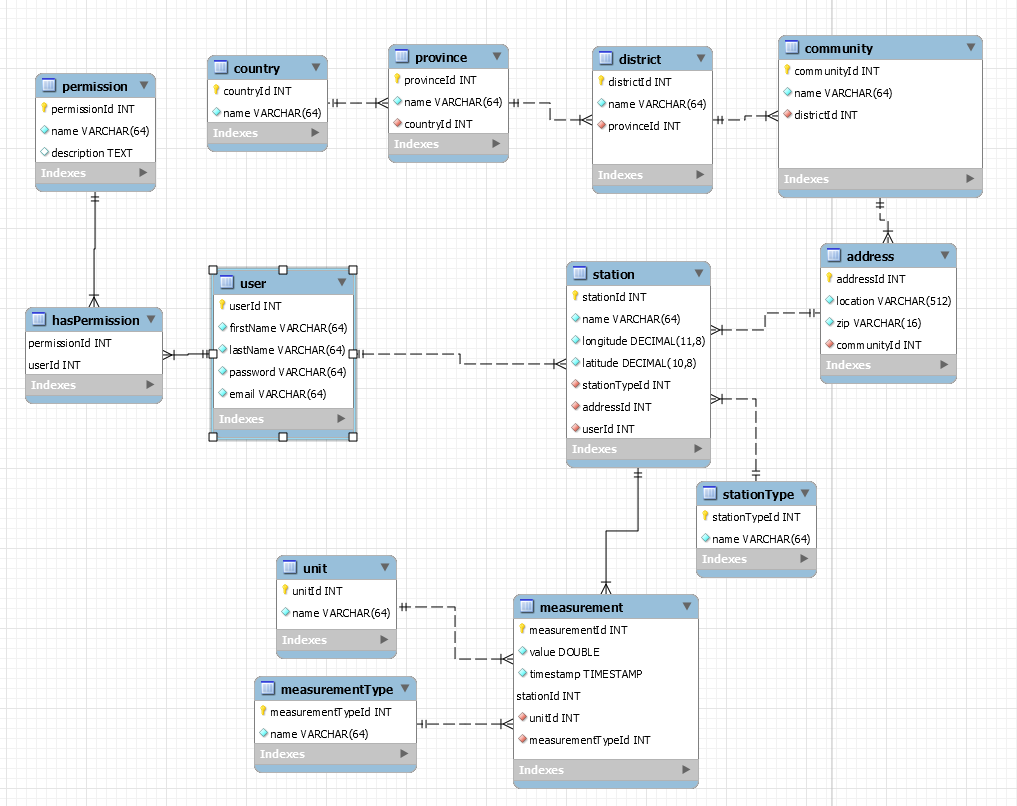
\includegraphics[width=.85\textwidth]{database.png}
\caption{Datenbankschema des Wetr-Projekts in der ersten Ausbaustufe.}
\label{fig:db}
\end{figure}
\raggedright
Wie in Abbildung \ref{fig:db} zu sehen wird zur Verwaltung des Standortes einer Station eine Reihe von abhängigen Entitäten verwendet. Um die Flexibilität zu erhöhen wurde neben zusätzlich ein \textit{Country} modelliert. In einem \textit{Country} befinden sich \textit{Provinces}, welche Bundesländer darstellen. Jede \textit{Province} wird in mehrere \textit{Districts} unterteilt, ähnlich wie Bezirke. In jedem \textit{District} gibt es mehrere \textit{Communities}, welche mit Gemeinden vergleichbar sind. Als kleinste Entität in dieser Kette gibt es die \textit{Address}, welche einen einfachen String zur Angabe von genaueren Addressdaten (rein zur Anzeige oder falls anderswo benötigt) und eine Zuordnung mittels Postleitzahl enthält.\\
Im Datenbankschema gibt es \textit{User}, welche, falls benötigt, verschiedene \textit{Permissions} zugewiesen haben können. Ein \textit{User} kann mehrere \textit{Stations} betreiben, welche wiederum neben der \textit{Address} auch einen Namen und die Geokoordinaten in Form von Latitide und Longitude gespeichert hat. Der Typ der Station wurde in eine eigene Entität \textit{StationType} ausgelagert.\\
Jede \textit{Station} kann beliebig viele \textit{Measurements} generieren, welche neben den ebenfalls ausgelagerten Entitäten \textit{MeasurementType} und \textit{Unit}, auch einen Zeitstempel und dazugehörigen Messwert besitzen.\\

